
%--------------- Personalize your document here ---------------

\author{Emmanuel Rockwell} % Enter your name
\newcommand{\supervisorone}{Vincent Toups} % Enter your supervisor's name
\newcommand{\supervisortwo}{}% Leave it empty or enter your second supervisor's name 
\newcommand{\department}{UNIVERISTY OF NORTH CAROLINA -- CHAPEL HILL\\ Department of Biostatistics}
\newcommand{\exam}{BIOS 611 FINAL PROJECT}

\title{Pitchfork Analysis} %Enter the title of your report 
\date{November 2021} % insert a specific date	



\documentclass[a4paper,12pt]{article}
\usepackage[left=30mm,top=30mm,right=30mm,bottom=30mm]{geometry}
\usepackage{etoolbox} %required for cover page
\usepackage{booktabs}
\usepackage[usestackEOL]{stackengine}
\usepackage[T1]{fontenc}
\usepackage[utf8]{inputenc}
\usepackage{bm}
\usepackage{graphicx}
\usepackage{subcaption}
\usepackage{amsmath}
\usepackage{amsfonts}
\usepackage{mathtools}
\usepackage{xcolor}
\usepackage{float}
\usepackage{hyperref}
\usepackage[capitalise]{cleveref}
\usepackage{enumitem,kantlipsum}
\usepackage{amssymb}
\usepackage[square,numbers,sort]{natbib}
\usepackage[ruled,vlined]{algorithm2e}
\usepackage{listings}
%\usepackage{minted}
%\usemintedstyle{emacs}

%\renewcommand{\listingscaption}{Algorithm}
%\renewcommand{\listoflistingscaption}{List of Algorithms}


%\bibliographystyle{unsrtnat}

\hypersetup{
	colorlinks,
	linkcolor={black},
	citecolor={blue!50!black},
	urlcolor={blue!80!black}
}

\linespread{1}

\newtheorem{theorem}{Theorem}[section]
\graphicspath{{figures/}}	

%----------------------------------TITLE PAGE -----------------------------------
\makeatletter
\def\maketitle{
	\begin{center}\leavevmode
		\normalfont
		%\includegraphics[width=0.35\columnwidth]{queenslogo.pdf}
		\vskip 0.5cm   
		\textsc{\large \department}\\
		\vskip 1cm
		\includegraphics[width = 0.4\linewidth]{"unc_seal.png"}
		\vskip 1cm
		\rule{\linewidth}{0.2 mm} \\
		{\large \exam}\\[1 cm]
		{\huge \bfseries \@title \par}
		\vspace{1cm}
		\rule{\linewidth}{0.2 mm} \\[1.5 cm]
		
		\begin{minipage}[t]{0.45\textwidth}
			\begin{flushleft} \large
				\emph{Author:}\\
				\@author
			\end{flushleft}
		\end{minipage}
		\begin{minipage}[t]{0.45\textwidth}
			\begin{flushright} \large
				\ifdefempty{\supervisortwo}{\emph{Instructor:\\}}{\emph{Instructor:\\}}
				\supervisorone\\
				\ifdefempty{\supervisortwo}{}{\supervisortwo\\}
			\end{flushright}
		\end{minipage}
		\vfill
		{\Large \@date\par}
	\end{center}
	%\vfill
	%\null
	\cleardoublepage
}
\makeatother


%-------------------------------- ENDTITLE PAGE ----------------------------------

\begin{document}
	
	\pagenumbering{gobble}% Remove page numbers (and reset to 1)
	
	\maketitle
	
	\tableofcontents

	\newpage
	%\listoffigures
	%\newpage
	%\listoftables
	%\newpage
	%\listofalgorithms % List of algorithms in pseudocode format
	%\newpage
	%\listoflistings % List of algorithms in code format
	%\newpage
	
	
	\pagenumbering{arabic}% Arabic page numbers (and reset to 1)
	
	% This is how you can organize your document
\section{Introduction}
Founded in 1995, Pitchfork is an online music \& culture website that also organized the annual Pitchfork Music Festival in Chicago, IL. However, Pitchfork is mainly known for it's album reviews. Rather than assigning some amount of stars, thumbs-up, or tomatoes, Pitchfork aims to pursue a further degree of objective precision to its reviews -- assigning to each album a score on a 101-point scale between 0.0 and 10.0. 

Pitchfork's brand has evolved over the years. For the first 20 years or so of its existence, Pitchfork was mostly a mainstay of more alternative and underground music scenes, developing a reputation a reputation for it's somewhat contrarian opinions regarding popular music. However, in 2015 Pitchfork was sold to the media conglomerate Conde Nast and with the acquisition morphed into a mouthpiece for the music industries top record labels. 

To analyze Pitchfork's reviews, I used a dataset from components.one that scraped every pitchfork review between 1999 and January, 2019. 



\section{Score Distributions}
\subsection{Assessing Overall Distribution of Reviews}
Perhaps the most interesting aspect of Pitchfork's reviews is the 101-point scale along which each album is evaluated. While this scale attempts to achieve a semblance of objectivity in reviews, very little is known about the methodology used when scores are assigned. Can we expect the average score to be a 5.0? What distribution of scores should we expect? How rare are very high and very low scores? Pitchfork doesn't disclose any of this information, so we're left to analyze the data ourselves to understand what the distribution of scores look like. Figure 1 shows the general distribution of the scores.

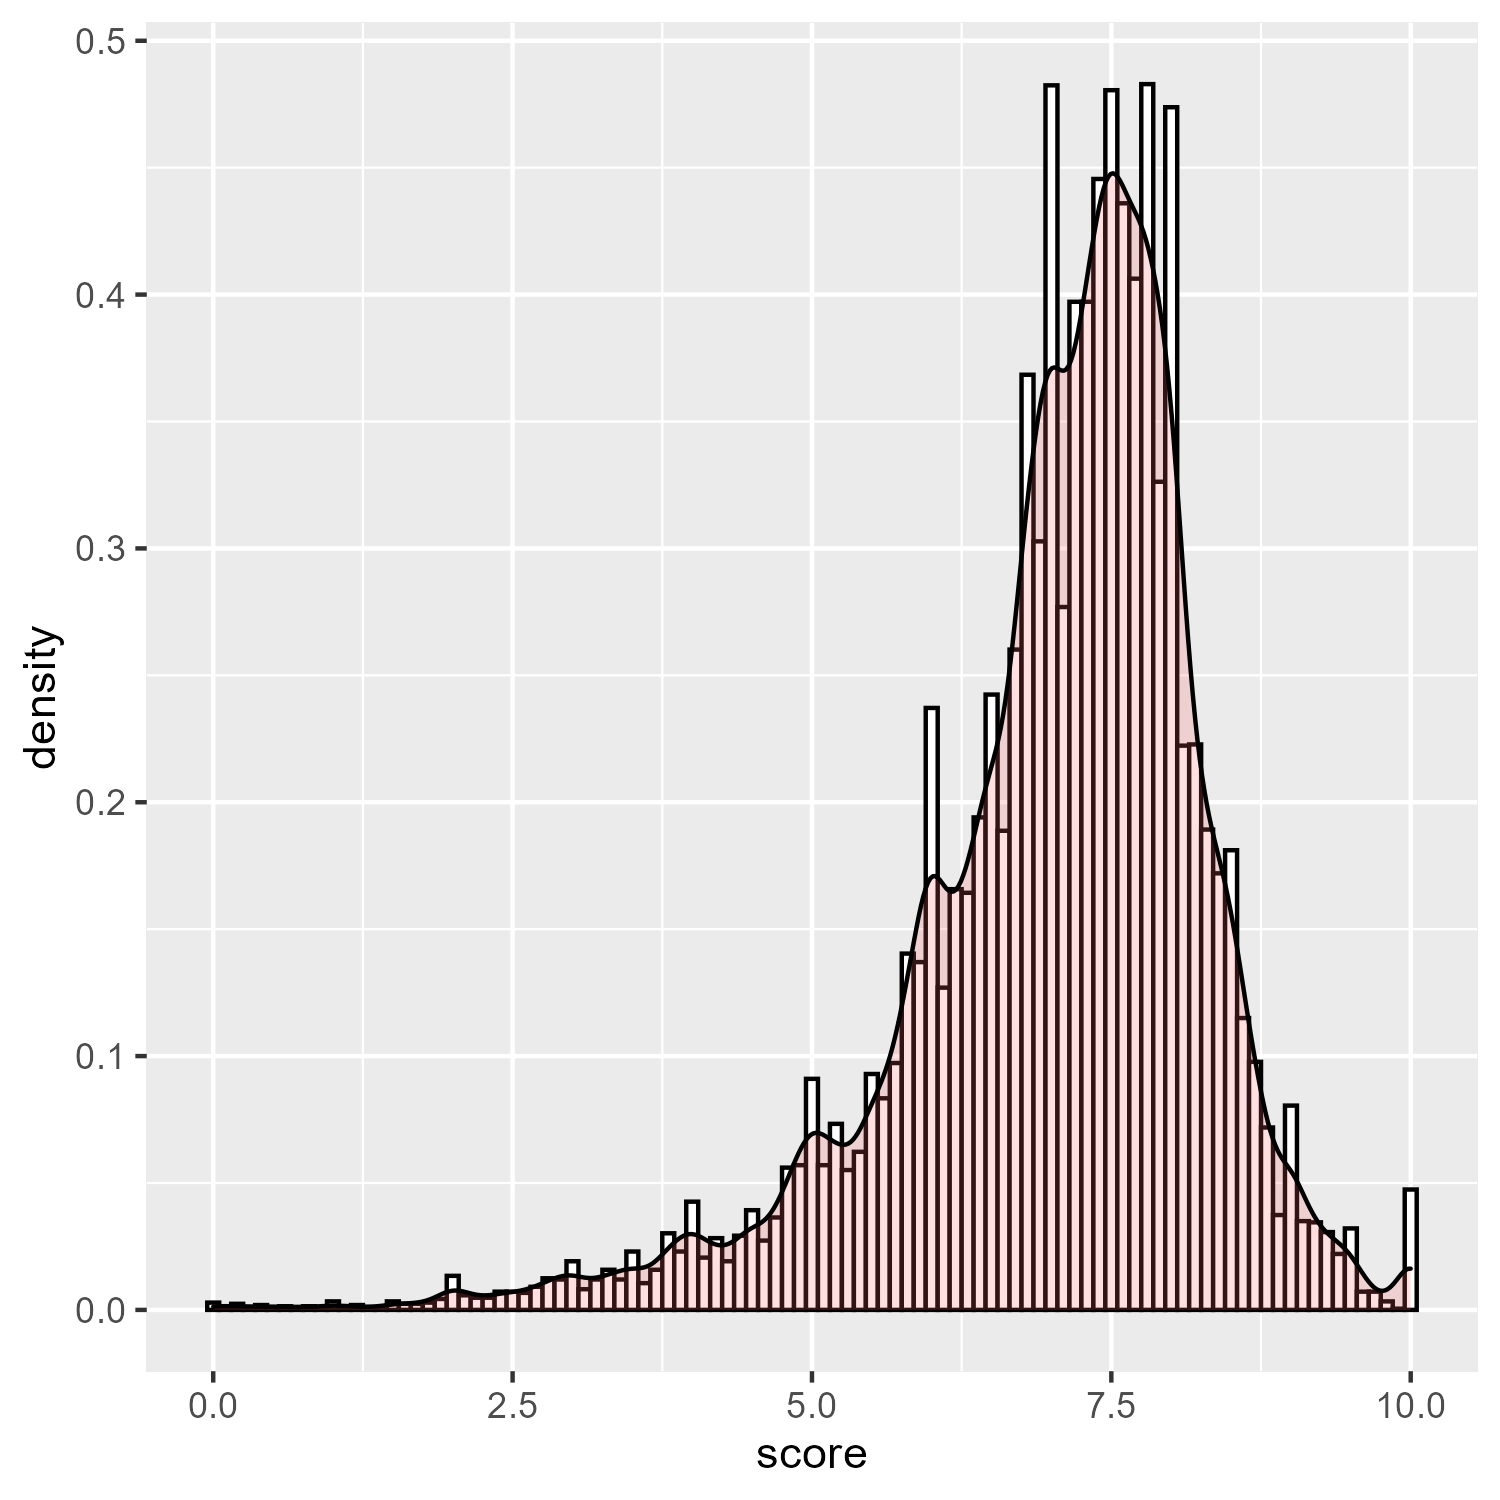
\includegraphics[width = 0.95\linewidth]{"figures/score_distribution.png"}

As we can see, scores seem to follow a left-skewed normal distribution. The mean score is 7.04 and the median score is 7.3. Therefore, a score is below-average and therefore "bad" relative to other albums if it has a score less than 7. A significant difference from the implicit assumption that 5 is the mean score. If this were the aim of the publication, they should attempt to be less favorable in their reviews. 
\subsection{Evaluating Score Objectivity}
Next I'd like to look at some interesting trends within the histogram -- specifically certain scores that are underindexed and overindexed empirically compared to what we would assume the theoretical distribution. 

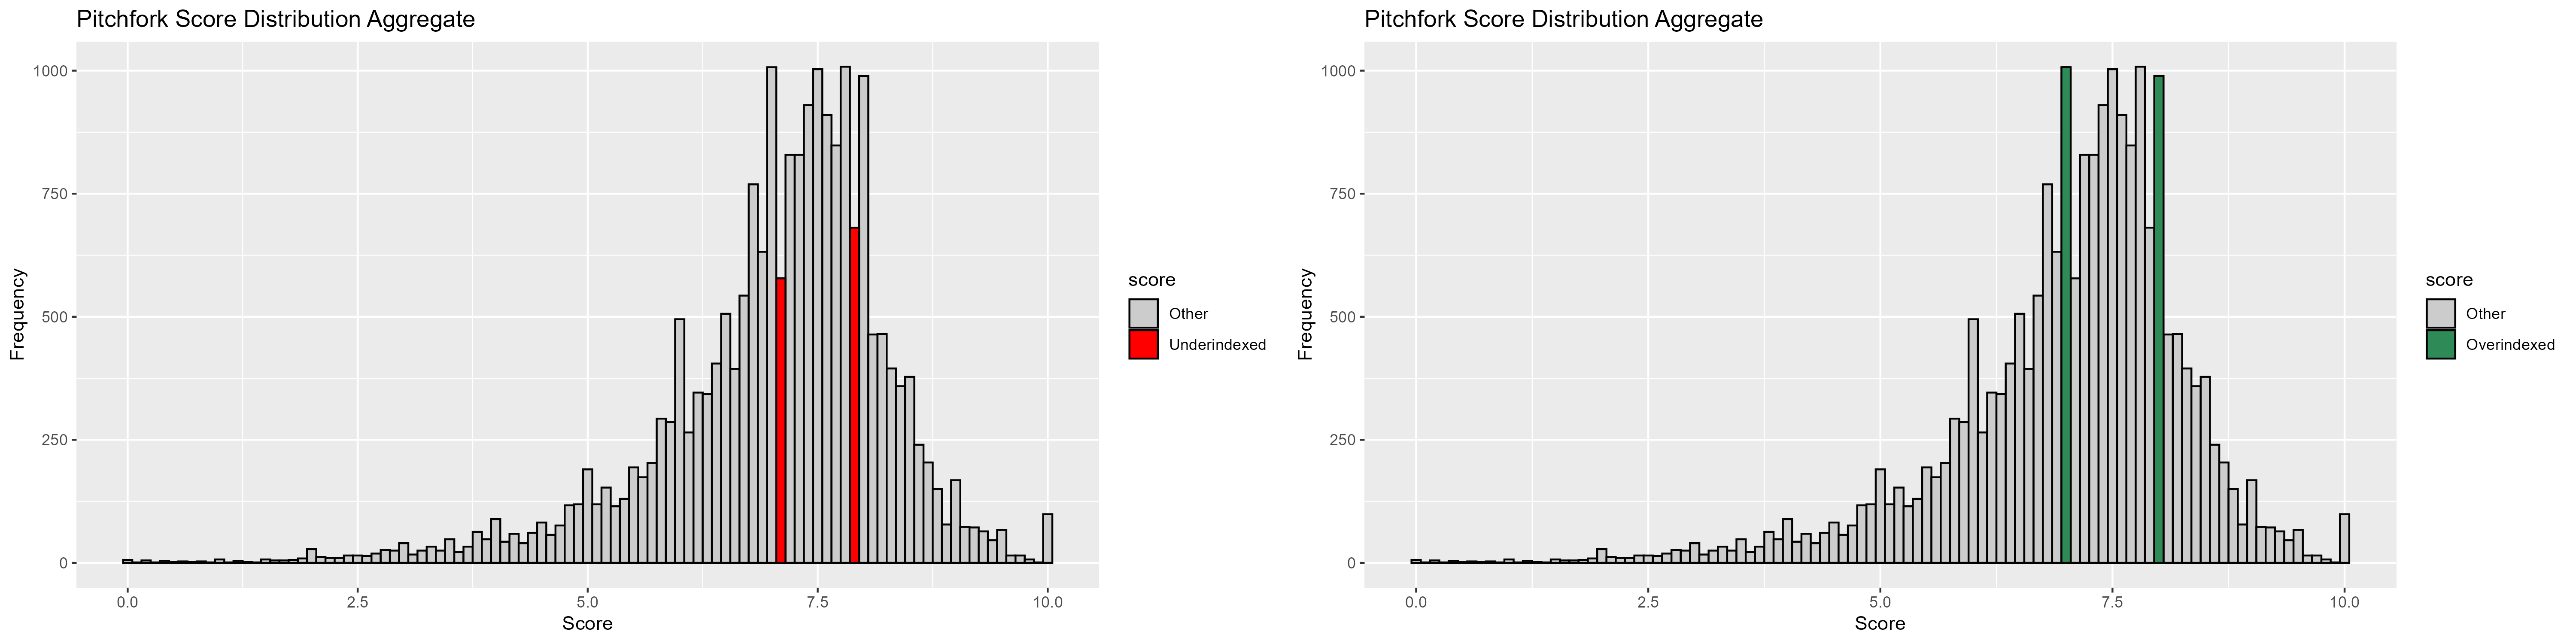
\includegraphics[width = \linewidth]{"figures/underoverindexing.png"}

The above figure highlights certain scores more or less prevalent in the empirical distribution than one would expect to find. Curiously, round numbers seem to be the most overindexed, with 7.0 and 8.0 both nearly matching the mode. On the other hand, scores like 7.1 and 7.9, while closer to the mode than 7.0 and 8.0, are significantly underrepresented in the data. Perhaps this reveals the more "human" aspect of this scoring convention. Since 7.1 and 7.9 seem like numbers that "lead" to 7.0 and 8.0 respectively, it appears that writers will unconsciously round down or round up when evaluating albums. 

\subsection{Distribution by Genre}

Finally, let's take a look at score distributions by genre. Pitchfork assigns multiple genres to albums -- often with many of the secondary genres being obscure. I simplified the issue by only taking the first genre listed on the website. This assumes that the first genre listed is the "primary" genre, which I believe is a fair assumption. 

I first wanted to understand whether Pitchfork writes more favorable reviews for certain genres. One can measure this by calculating the average score by genres and seeing how much this differs from the average score of 7.04. Furthermore, do the distribution of scores for specific genres differ significantly from the overall distribution? The below figures attempt to answer these questions: 

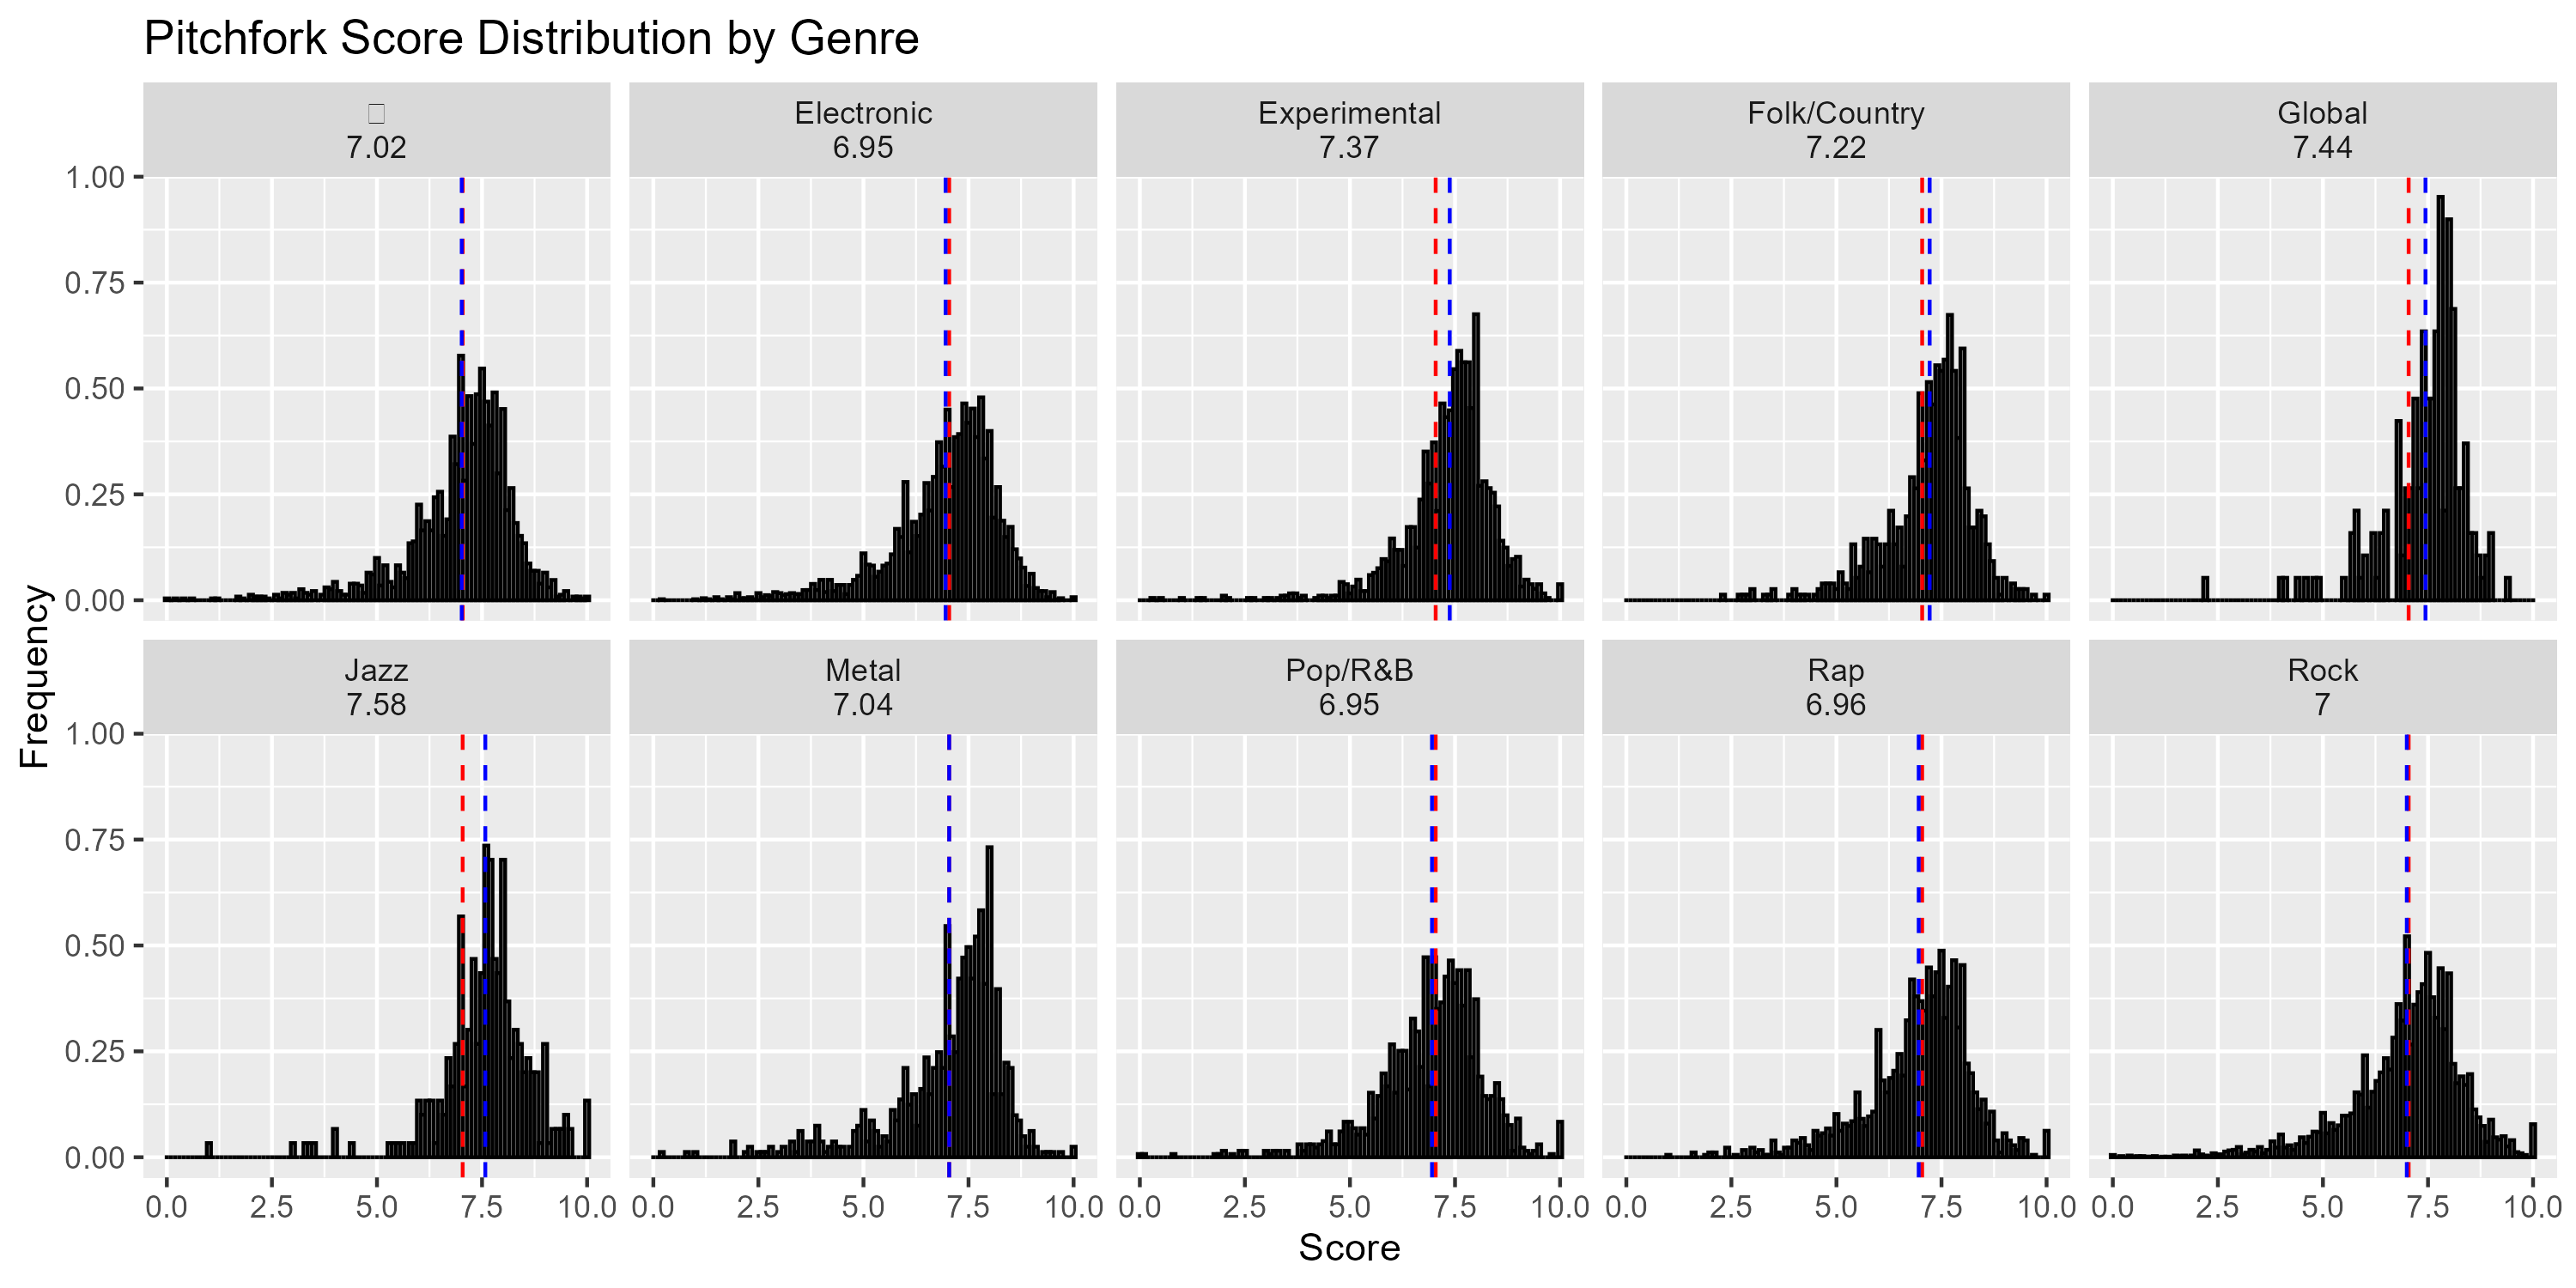
\includegraphics[width = 0.95\linewidth]{"figures/score_dist_by_genre.png"}

Note that the first histogram represents all albums without a listed genre. Albums with no genre represented about 10\% of albums and the average rating on these albums was consistent with the overall average. Pitchfork apparently provides higher scores on average to Jazz, Global, Experimental, and Folk/Country albums. On the other hand, Pitchfork gives it's least favorable reviews (on average) to Pop/R\&B, Electronic, and Rap albums. However, the low scores on these albums appear to be due to a longer tail than the Jazz, Global, Experimental, and Folk/Country album distributions. Therefore, I would conclude that Pitchfork likely doesn't rate these albums lower on average, but rather has a lower threshold for what constitutes being worthy of review.

\section{The Contrarian Index - Pitchfork vs. Popular Music}
\subsection{Historical Background}
In its early years, Pitchfork build a reputation of having somewhat contrarian opinions regarding popular music. During this time, Pitchfork grew its brand by not guaranteeing that most successful or most well-known albums receive the highest ratings -- distinguishing Pitchfork from other music and culture review publications. However, in 2015 Pitchfork was acquired by mega-conglomerate publisher Conde Nast, becoming a facet of the music industry it had formerly opposed. I'd like to see whether this historical reputation is backed by the data.

\subsection{Formulating the Contrarian Index}
There are many approaches that could be taken in formulating an index of contrarian reviews. However, I think the most straightforward approach would be to look at the disparity between the average Pitchfork reviews, and the average review of popular albums. 

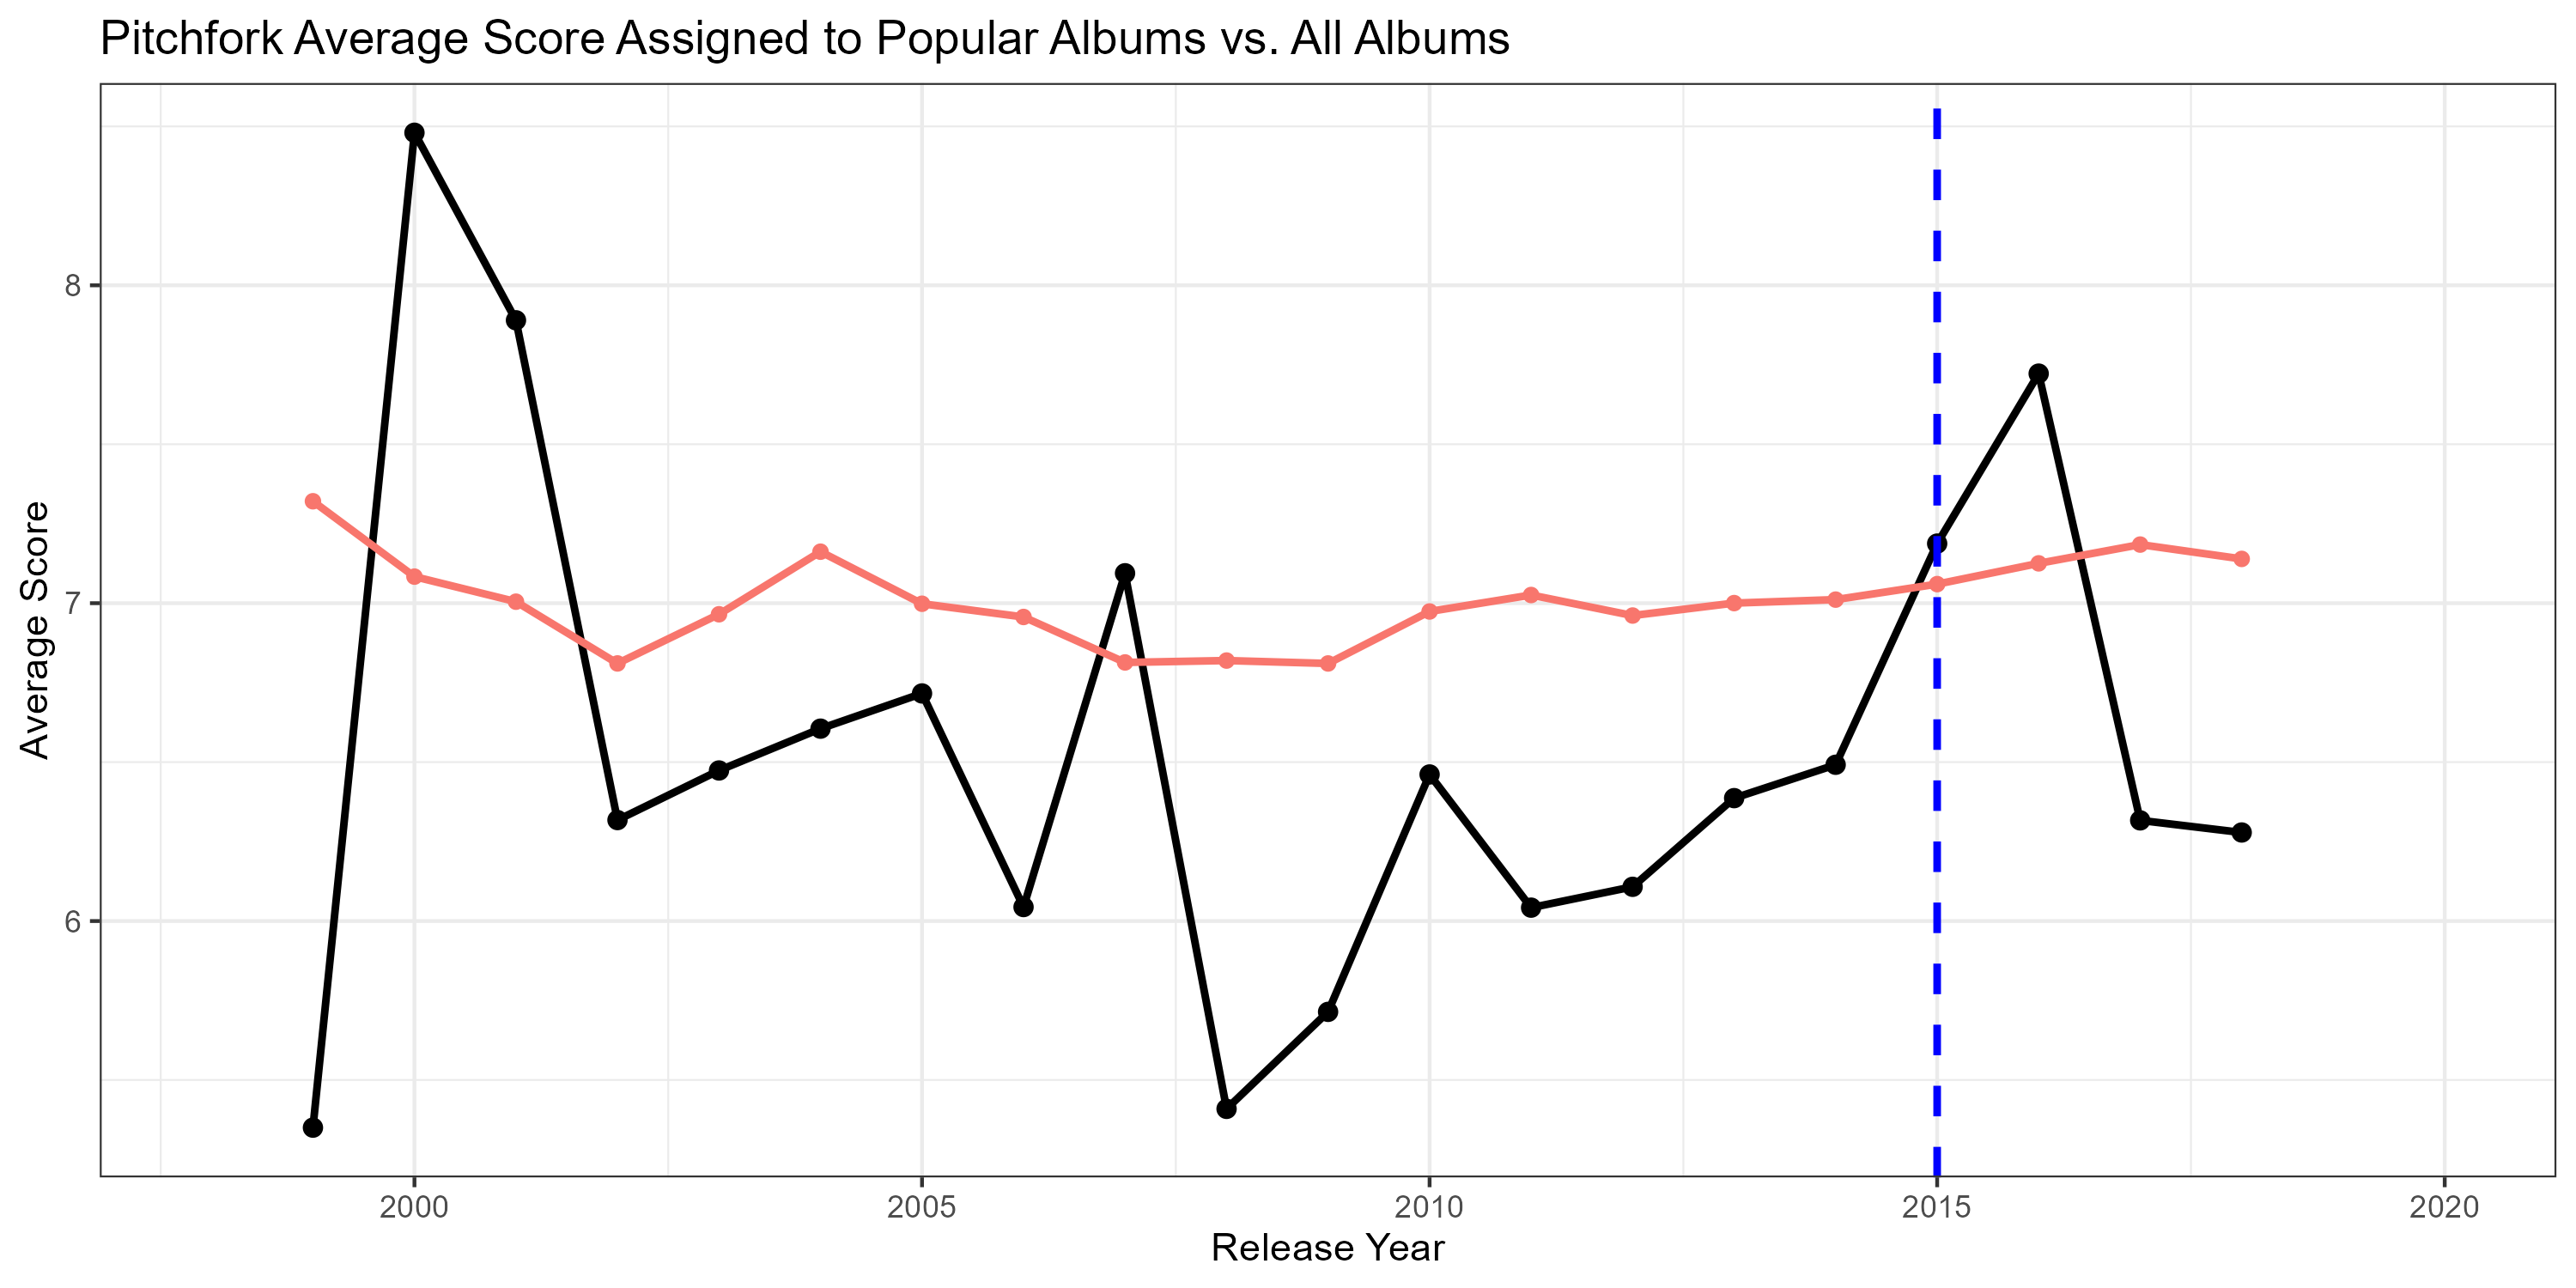
\includegraphics[width = 0.95\linewidth]{"figures/contrarian_index.png"}

The average score of pitchfork reviews by year is shown in red. The average Pitchfork review of albums who met certain Record Industry Association of America (RIAA) certifications (i.e. gold, diamond, platinum, and multi-platinum albums) is displayed in black. The blue line represents the year of the Conde Nast acquisition.

We can see that Pitchfork began by giving very favorable reviews to the top albums, but between 2002 and 2014 settled into giving below average reviews to the most successful albums. However, in 2015 -- the same year Pitchfork was acquire by Conde Nast -- it began giving much more favorable reviews to popular albums. The only true enigma in the graph is low scores given to the most popular albums in recent years. Here is another view of the same information:

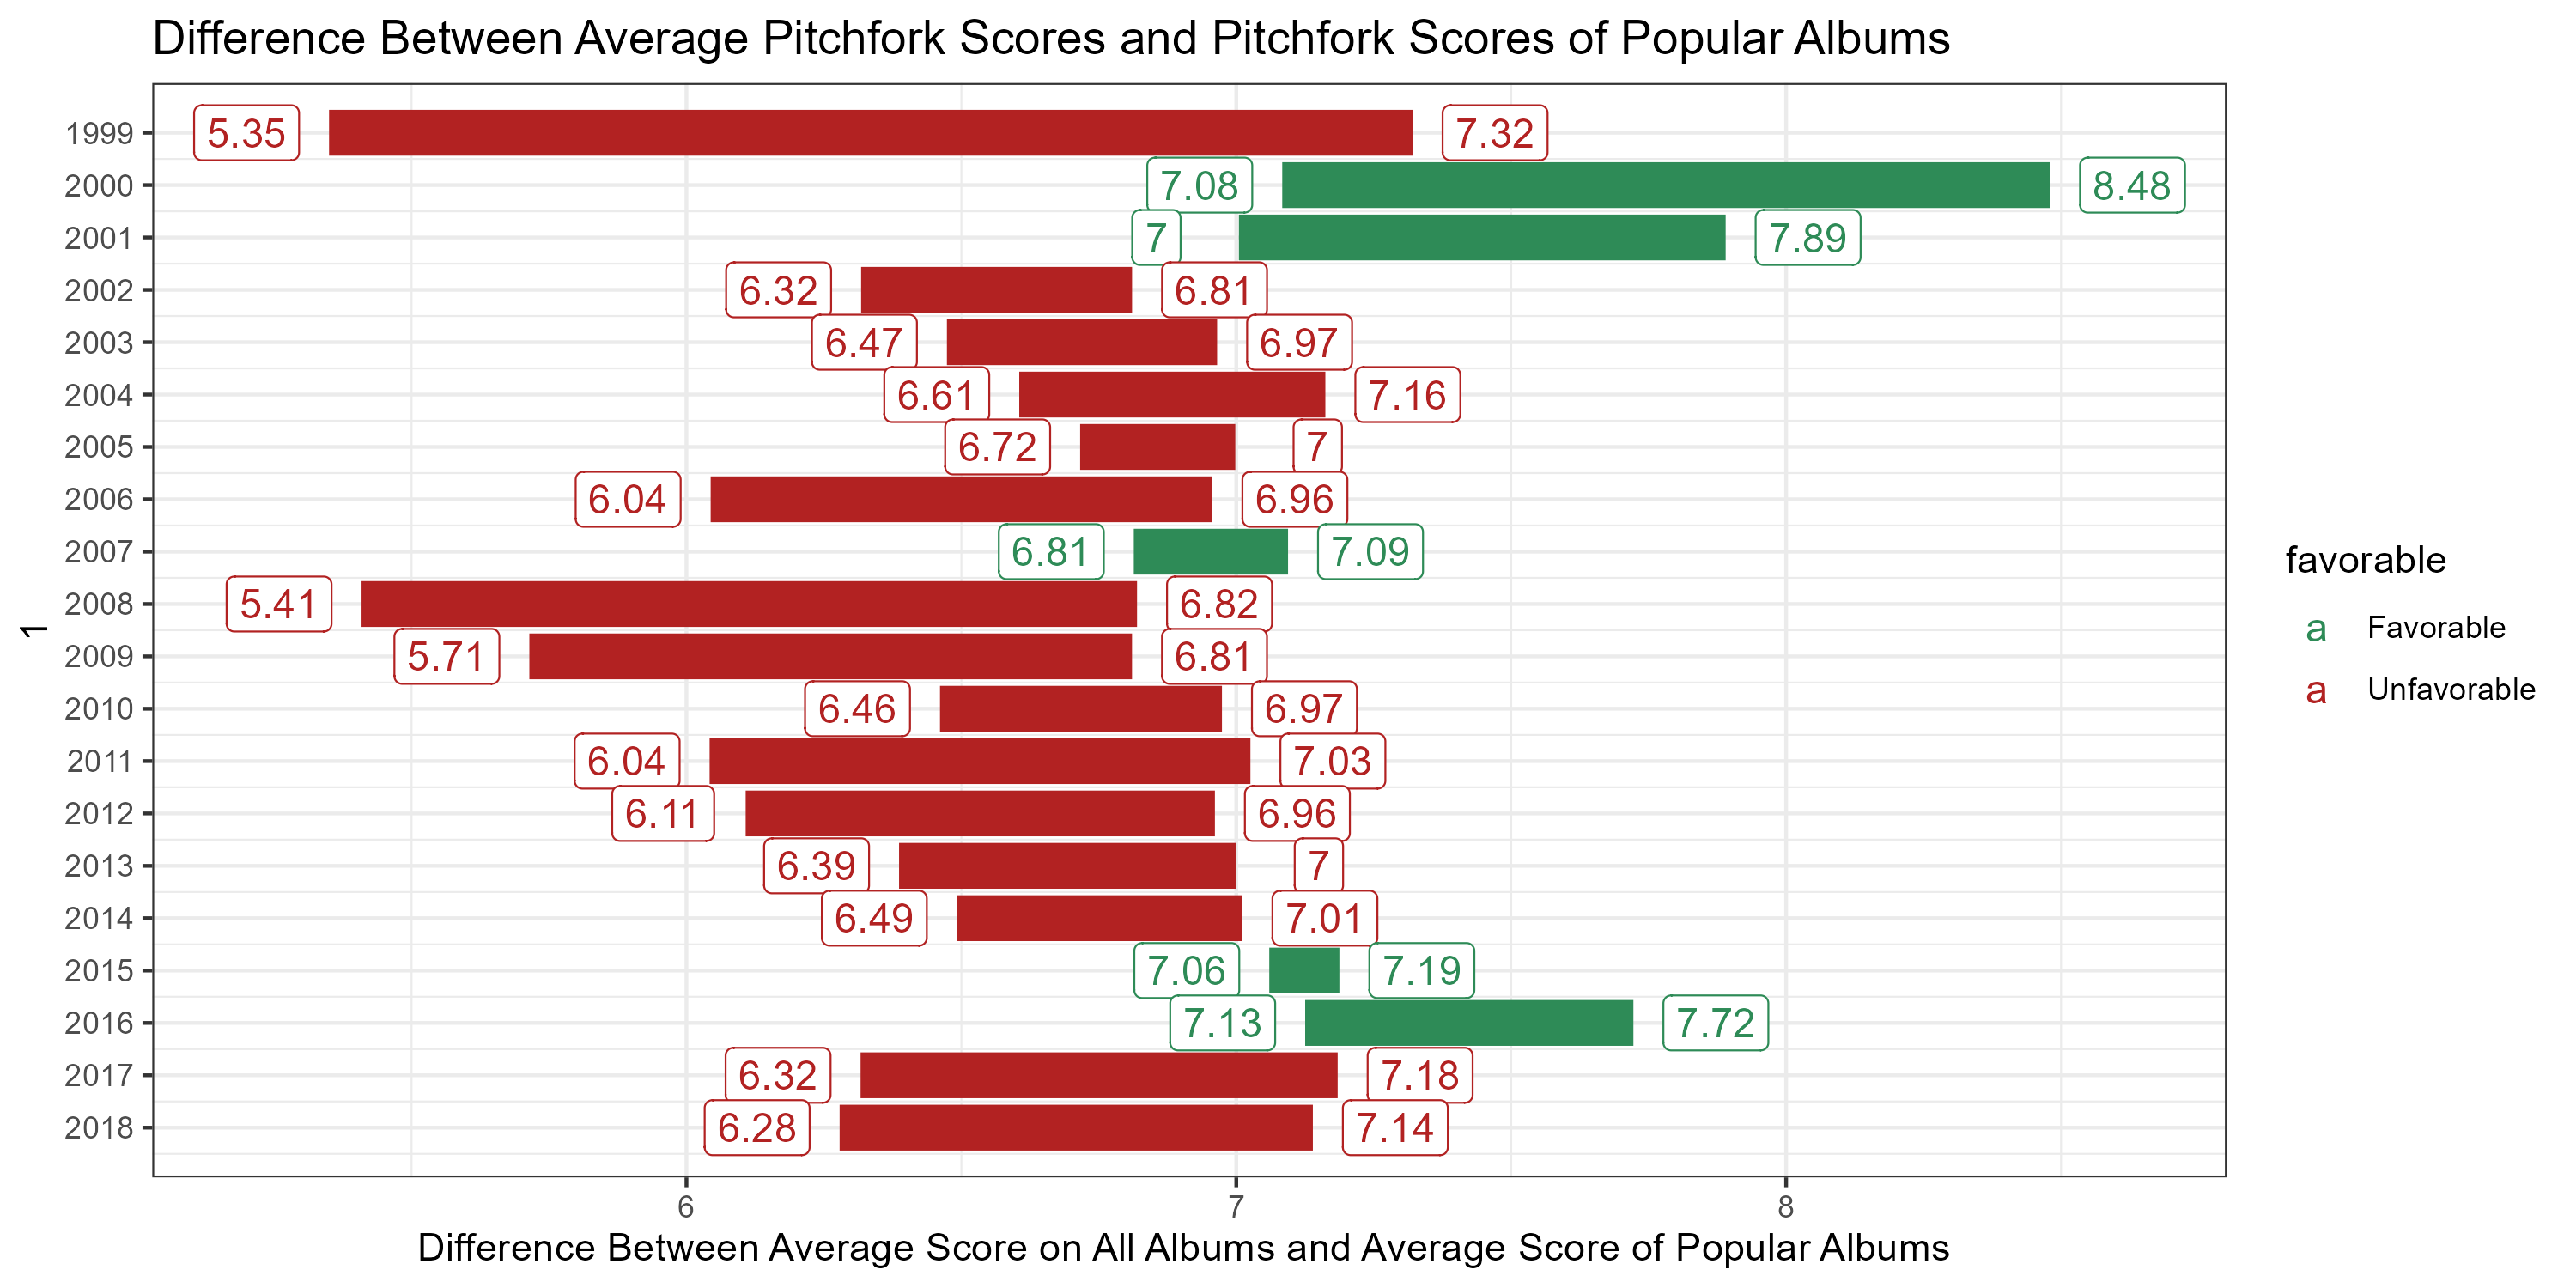
\includegraphics[width = \linewidth]{"figures/contrarian_index_bar.png"}

Going down the graph, we can see the degree to which the ratings of the most popular albums surpassed or fell short of the average rating by year. It's important to note that popular albums only constituted about 2\% of all Pitchfork reviews from year to year. Therefore, more variation should be expected. However, the decree to which these albums consistently under-perform compared to the average album at least partially confirms the suspicion that Pitchfork is biased against popular albums. 

\section{Album Review Text Mining}
\subsection{Preliminary Data Wrangling}
Perhaps the most interesting but unwieldy aspect of this dataset is it's content of reviews themselves. Each row contains the entire text (sometimes 10,000+ words) of the associated review of the album, presenting a very interesting opportunity in text mining and natural language processing. However, performing operations on 20,000+ reviews requires a good deal of processing power. Furthermore, looking at the average review might not be exceedingly interesting.

Luckily Pitchfork assigns it's favorite albums with its "best new music" label -- allowing me to subset the albums receiving the highest praise. I performed some text bagging and tallied the frequency of words within these reviews. While I did use a dictionary of common English stop words, I noticed that some of the most popular words were very standard words you would see to describe music, like "music," "album," "songs," "sound," and "record." These words aren't very informative of qualities unique to the best music, so I created an additional dictionary to remove these uninteresting words. 

\subsection{Evaluating Word Frequency in Good and Bad Reviews}
To understand the qualities of the most favorable reviews, I thought it might be useful to contrast the content of the worst reviews. While Pitchfork doesn't have a category for bad reviews, I can achieve something similar by taking all scores below a certain threshold. I chose 4.7 as my cutoff because it produced a similar number of observations as the good reviews, and I want to be comparing balanced data. Below are the top 20 words for good reviews when removing stopwords, the top 20 words for good review removing additional music-related words, and the top 20 words for bad review removing additional music-related words.

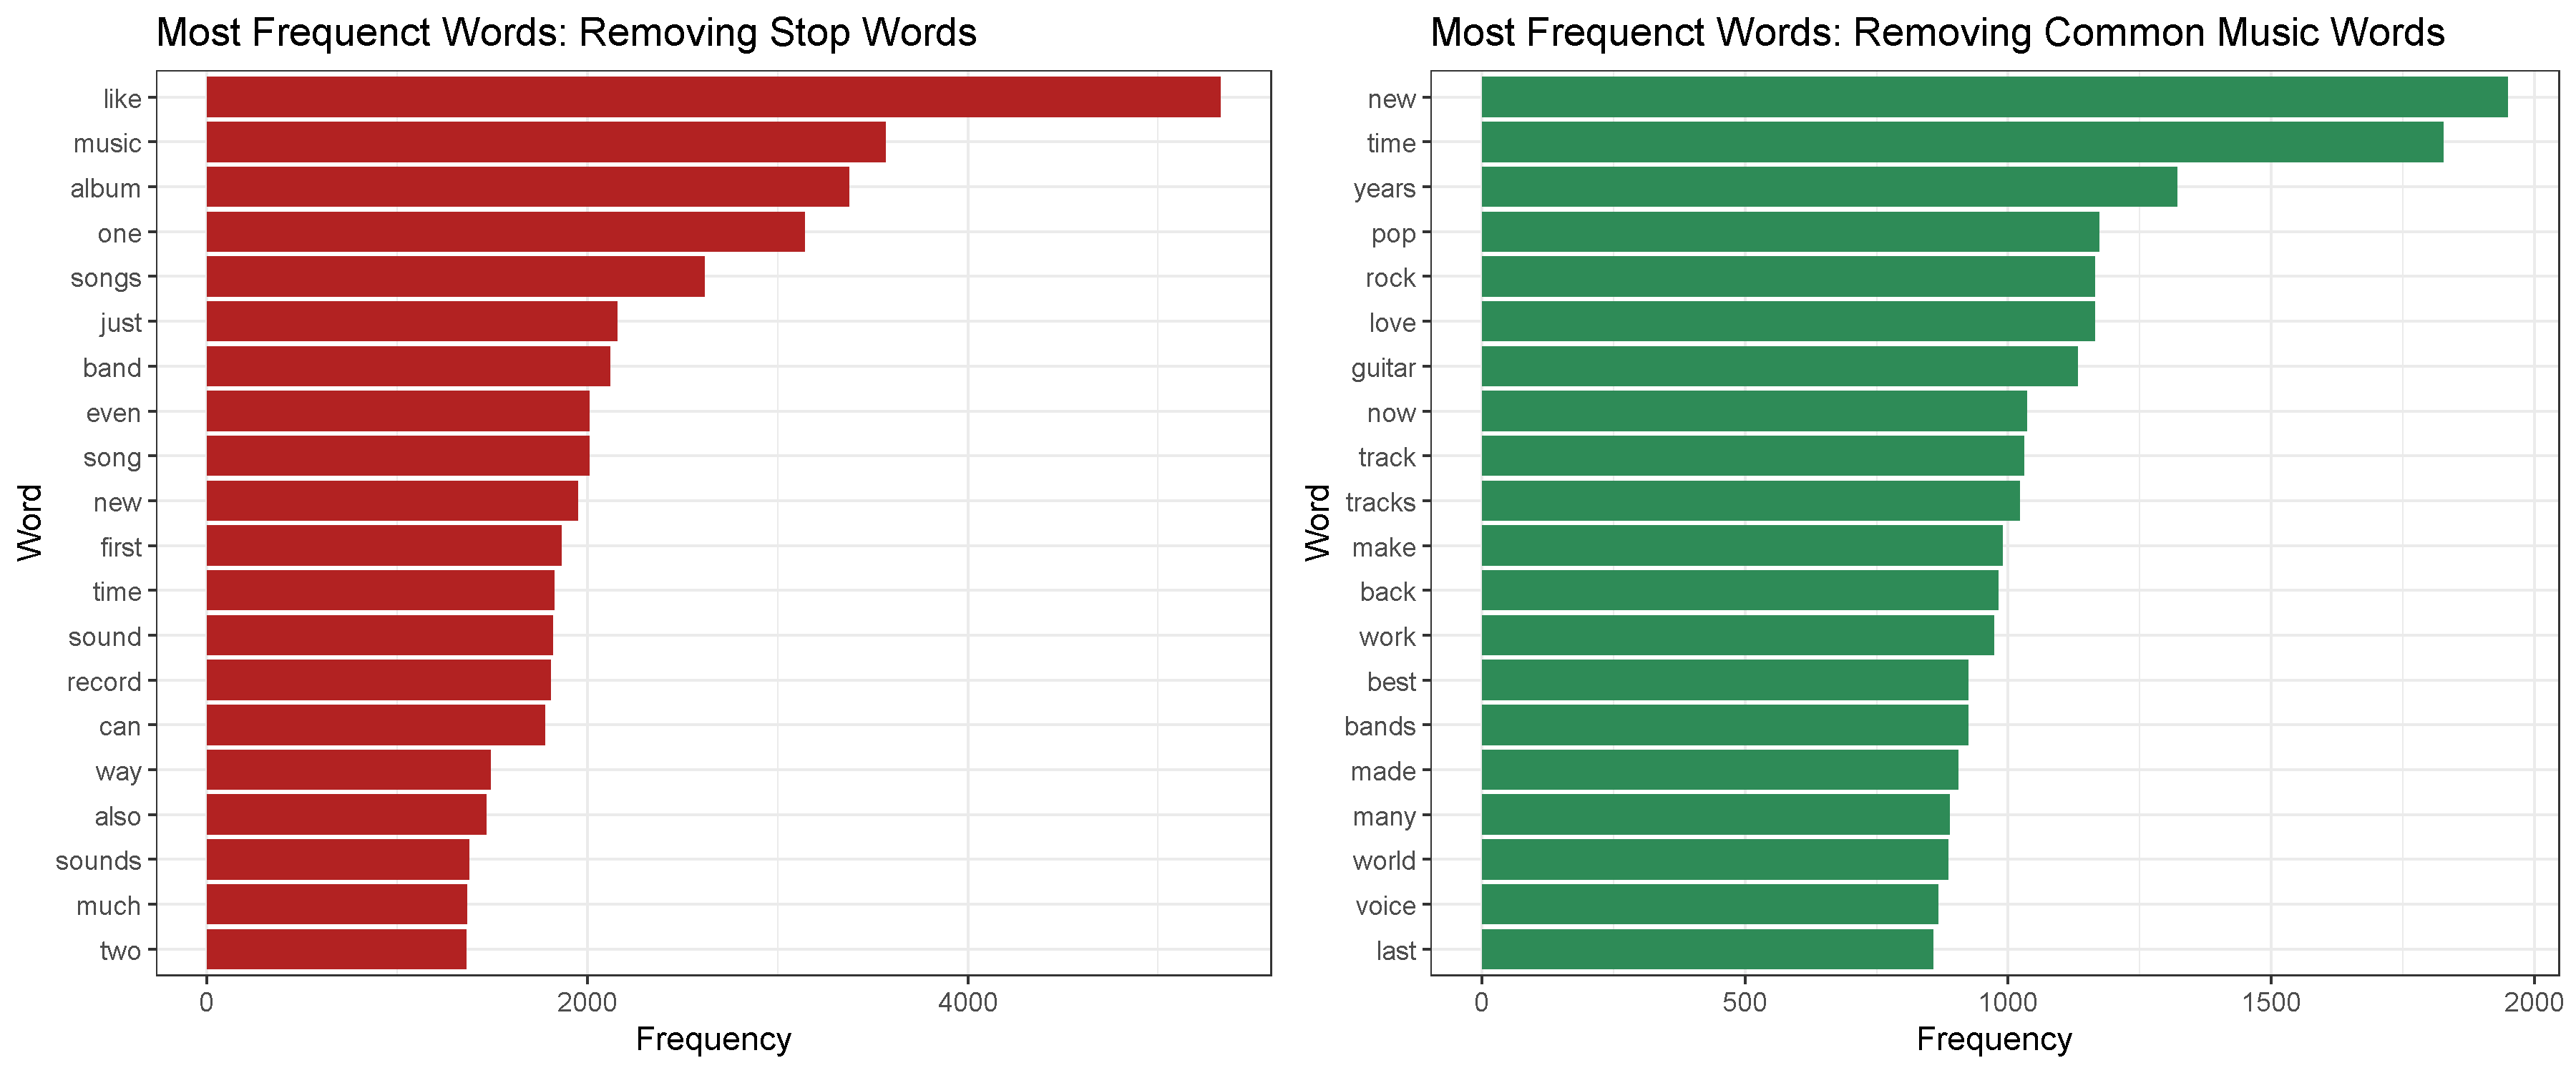
\includegraphics[width = 0.95\linewidth]{"figures/word_distribution_plot.png"}

The leftmost graph demonstrated how common music-related words are. Turning to the two rightmost graphs, it appears that the top words are somewhat similar. In both lists, "new" and "time" are the most commonly words in reviews. I suppose this isn't surprising since most albums are new at the time the review is written. 

However, making comparisons across these charts isn't easy. We can make it a bit easier to compare the relative ranks of works within good reviews and bad reviews with a different visualization:

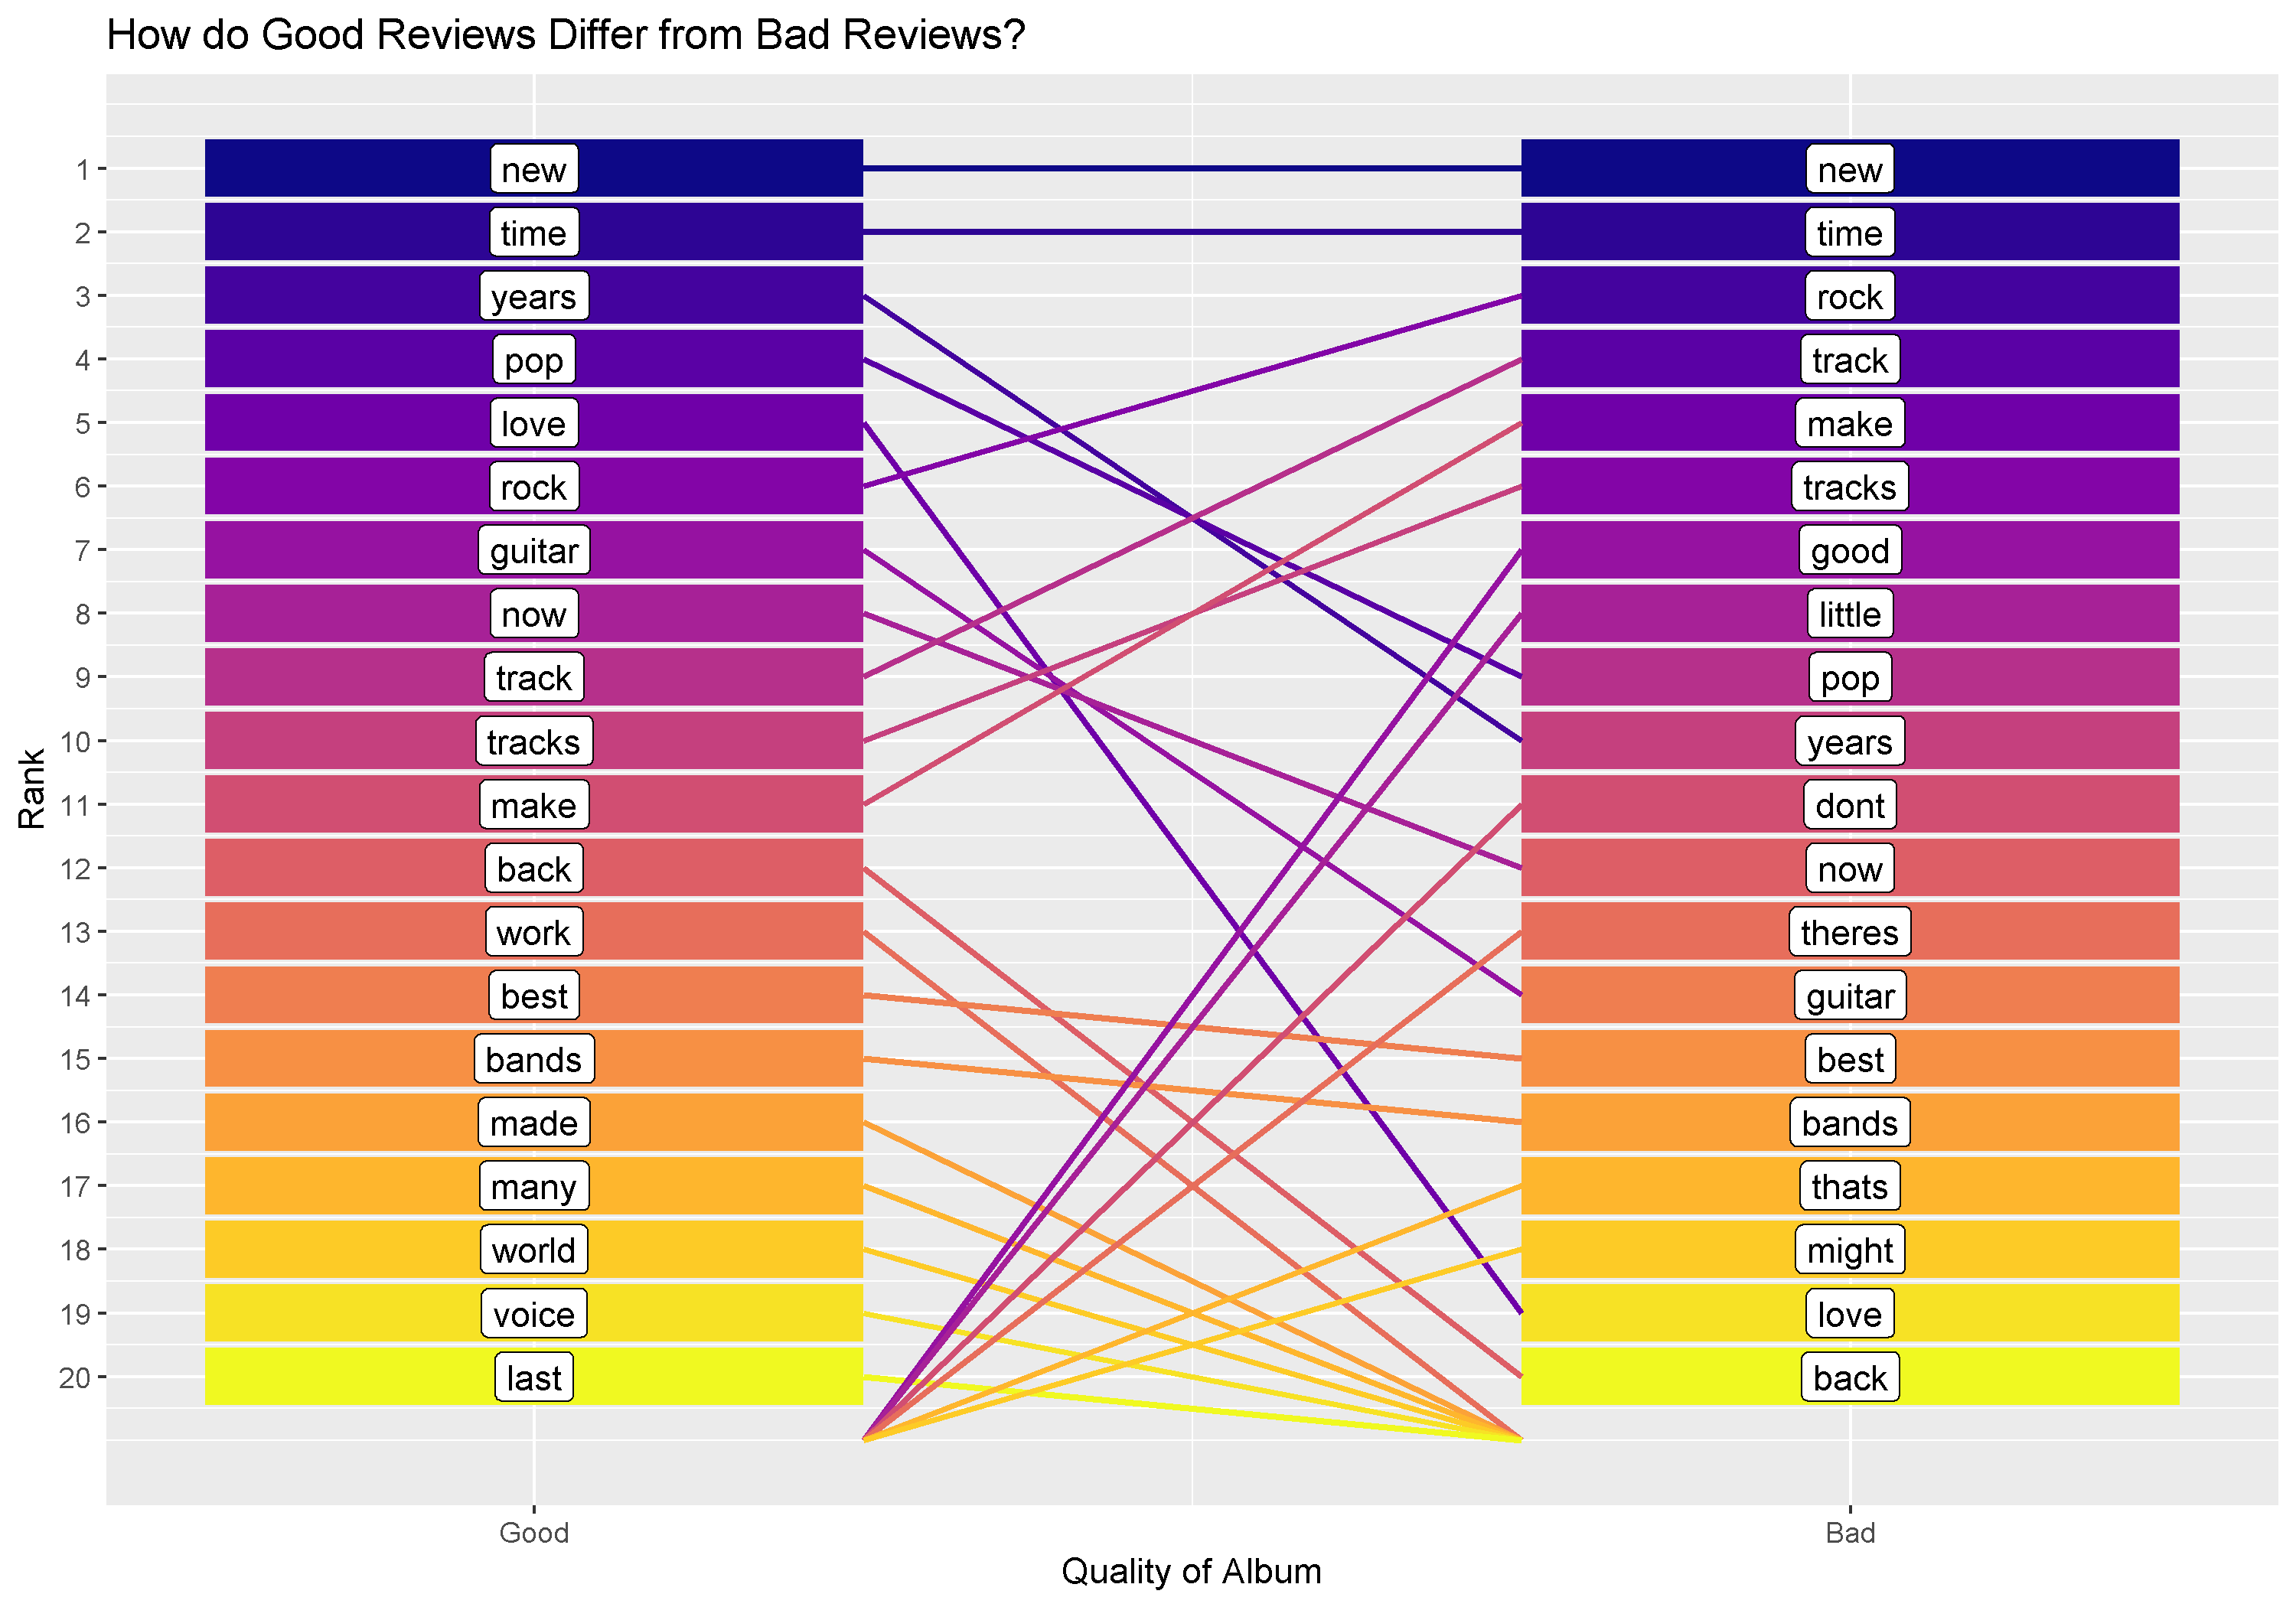
\includegraphics[width = 0.95\linewidth]{"figures/word_comparison.png"}

Here we can see that the word with the most significant difference in rank between the two category of review is "love." This is relatively straightforward (honestly I thought the disparity between words like "love" would be even greater). 

\subsection{Fun with Word Clouds}
Finally, I concluded my analysis of the content of reviews by creating word Clouds for both the favorable reviews and unfavorable reviews. Web versions of these word Clouds may be found withing the "figures" folder of my github repository, but a snapshot of their results is also provided on the next page. 

\section{Conclusion}
This analysis certainly isn't exhaustive. With more time, I'd love to continue analysis of this data to explore even more granular aspects of the content of these reviews, engage in predictive modeling efforts, and continue updating the dataset to contain the most recent reviews. Regardless, thank you for reading my paper. Any future updates can be found in my \href{https://github.com/mannyrockwell/bios-611-project}{my github repository}. 

\begin{center}
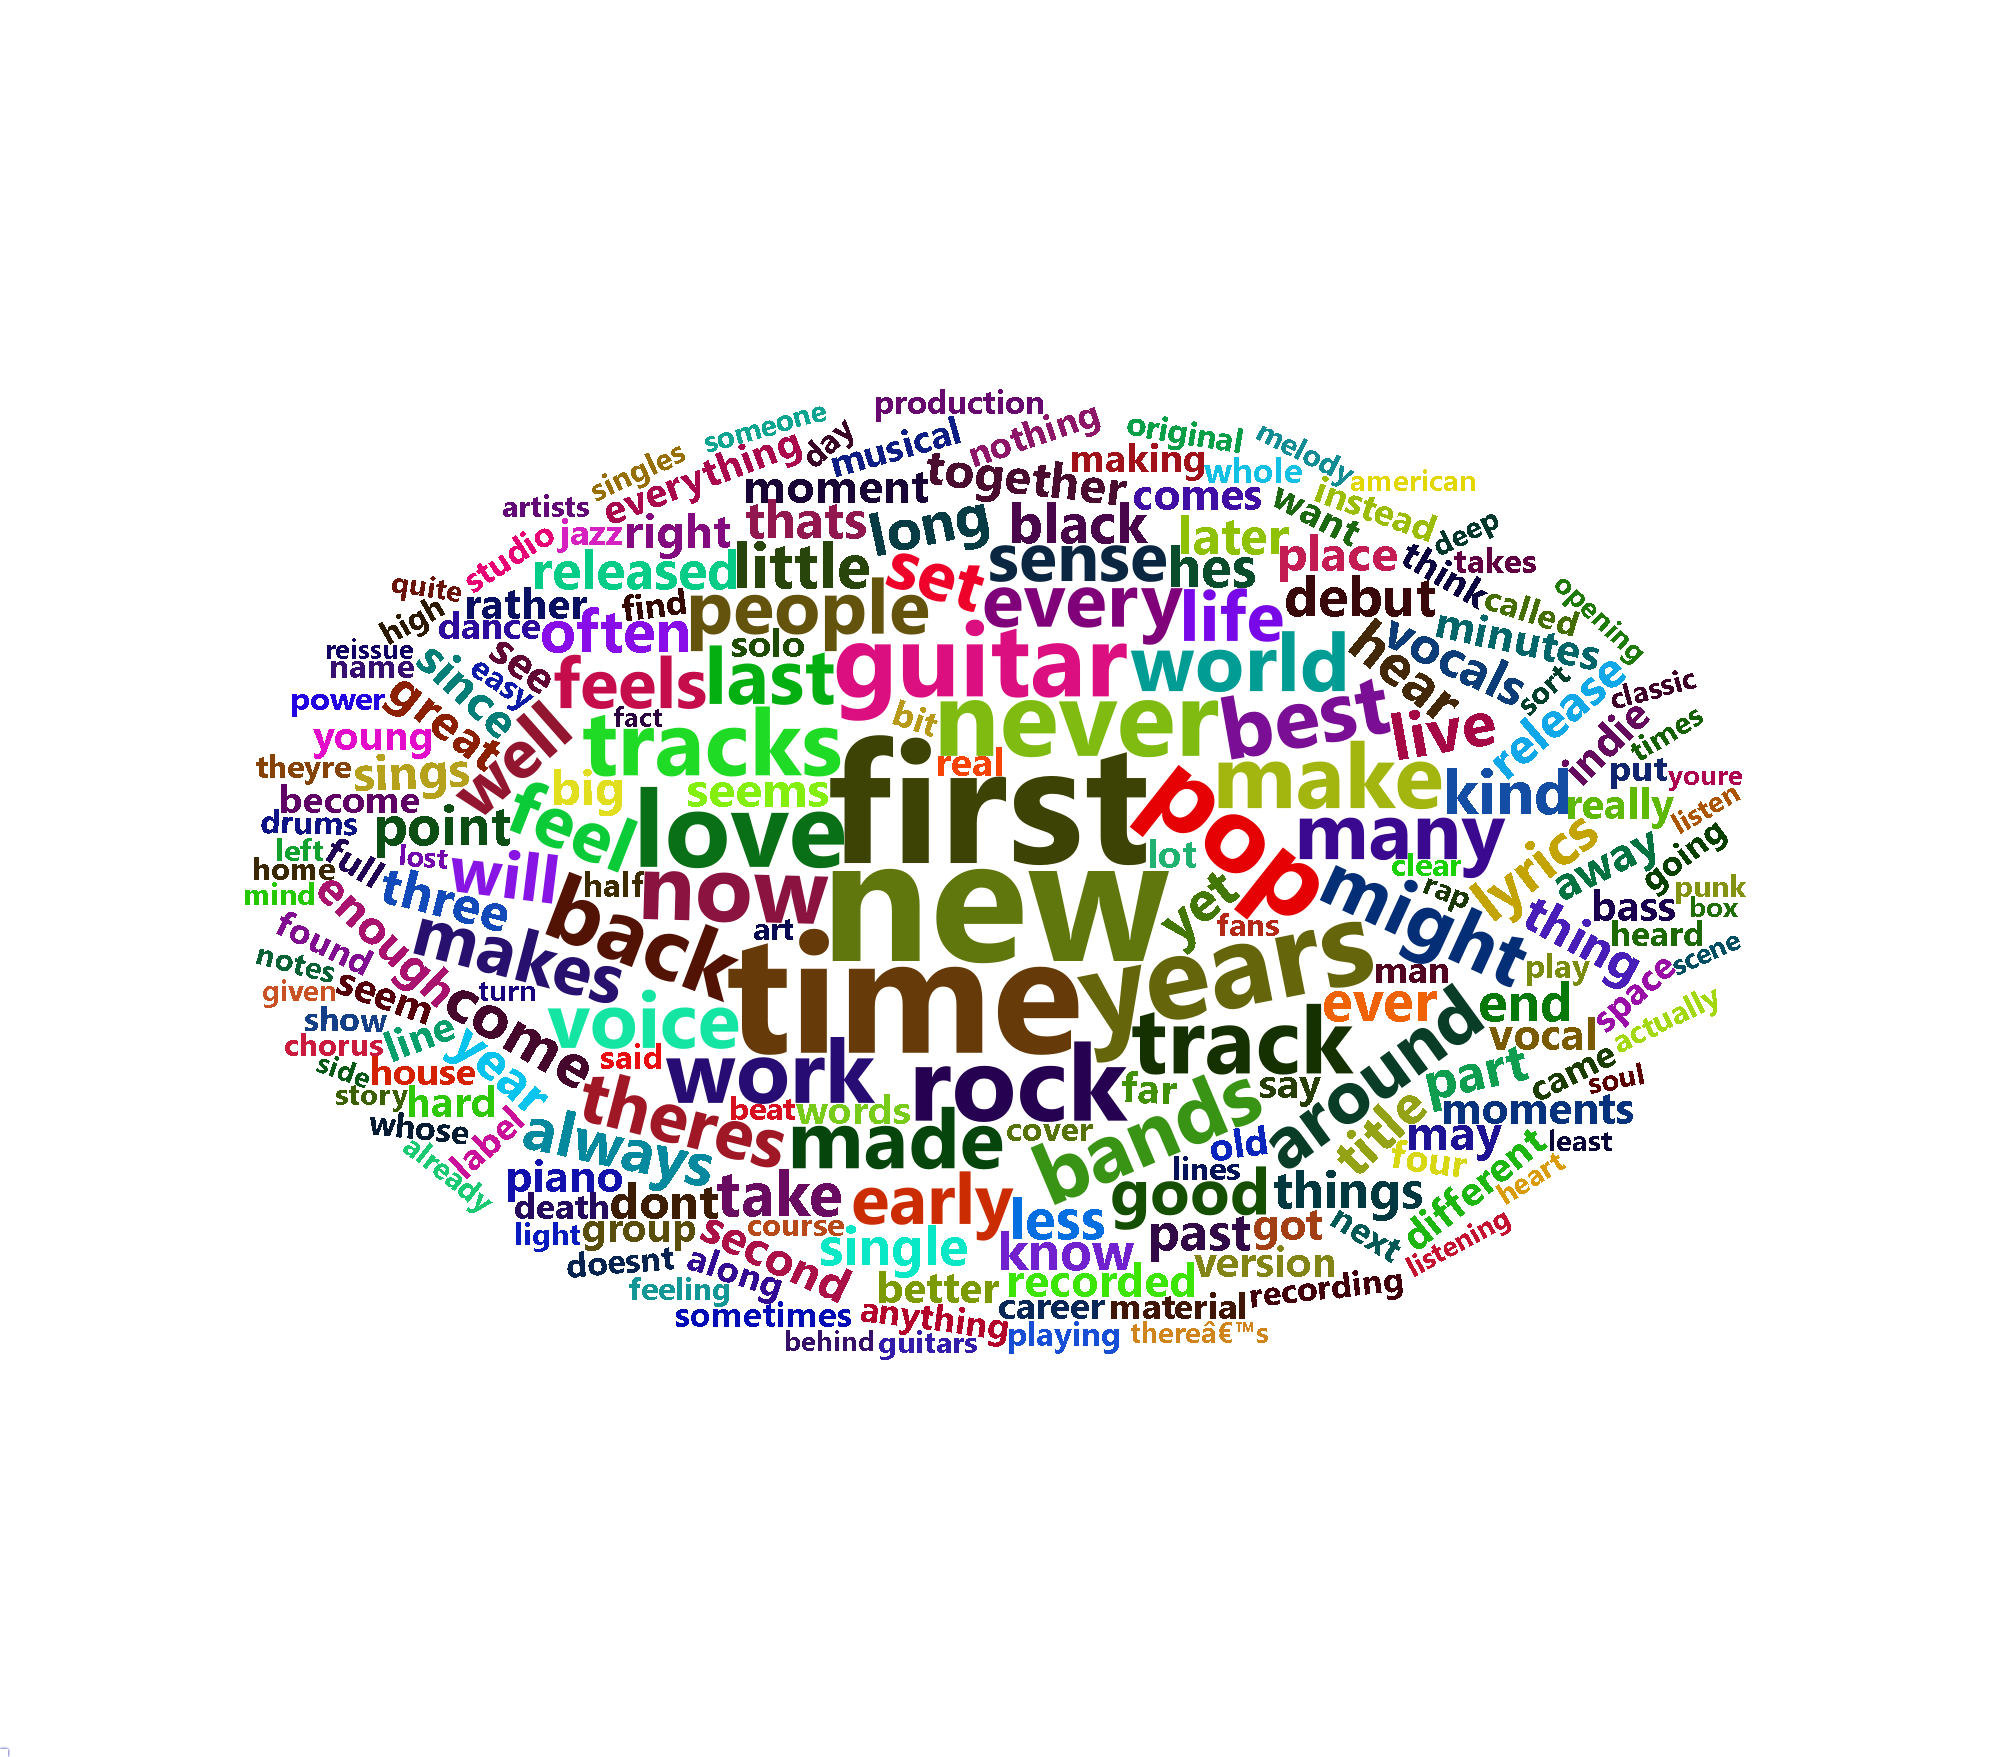
\includegraphics[width = \linewidth]{"figures/wordcloud.png"}
\end{center}
\begin{center}
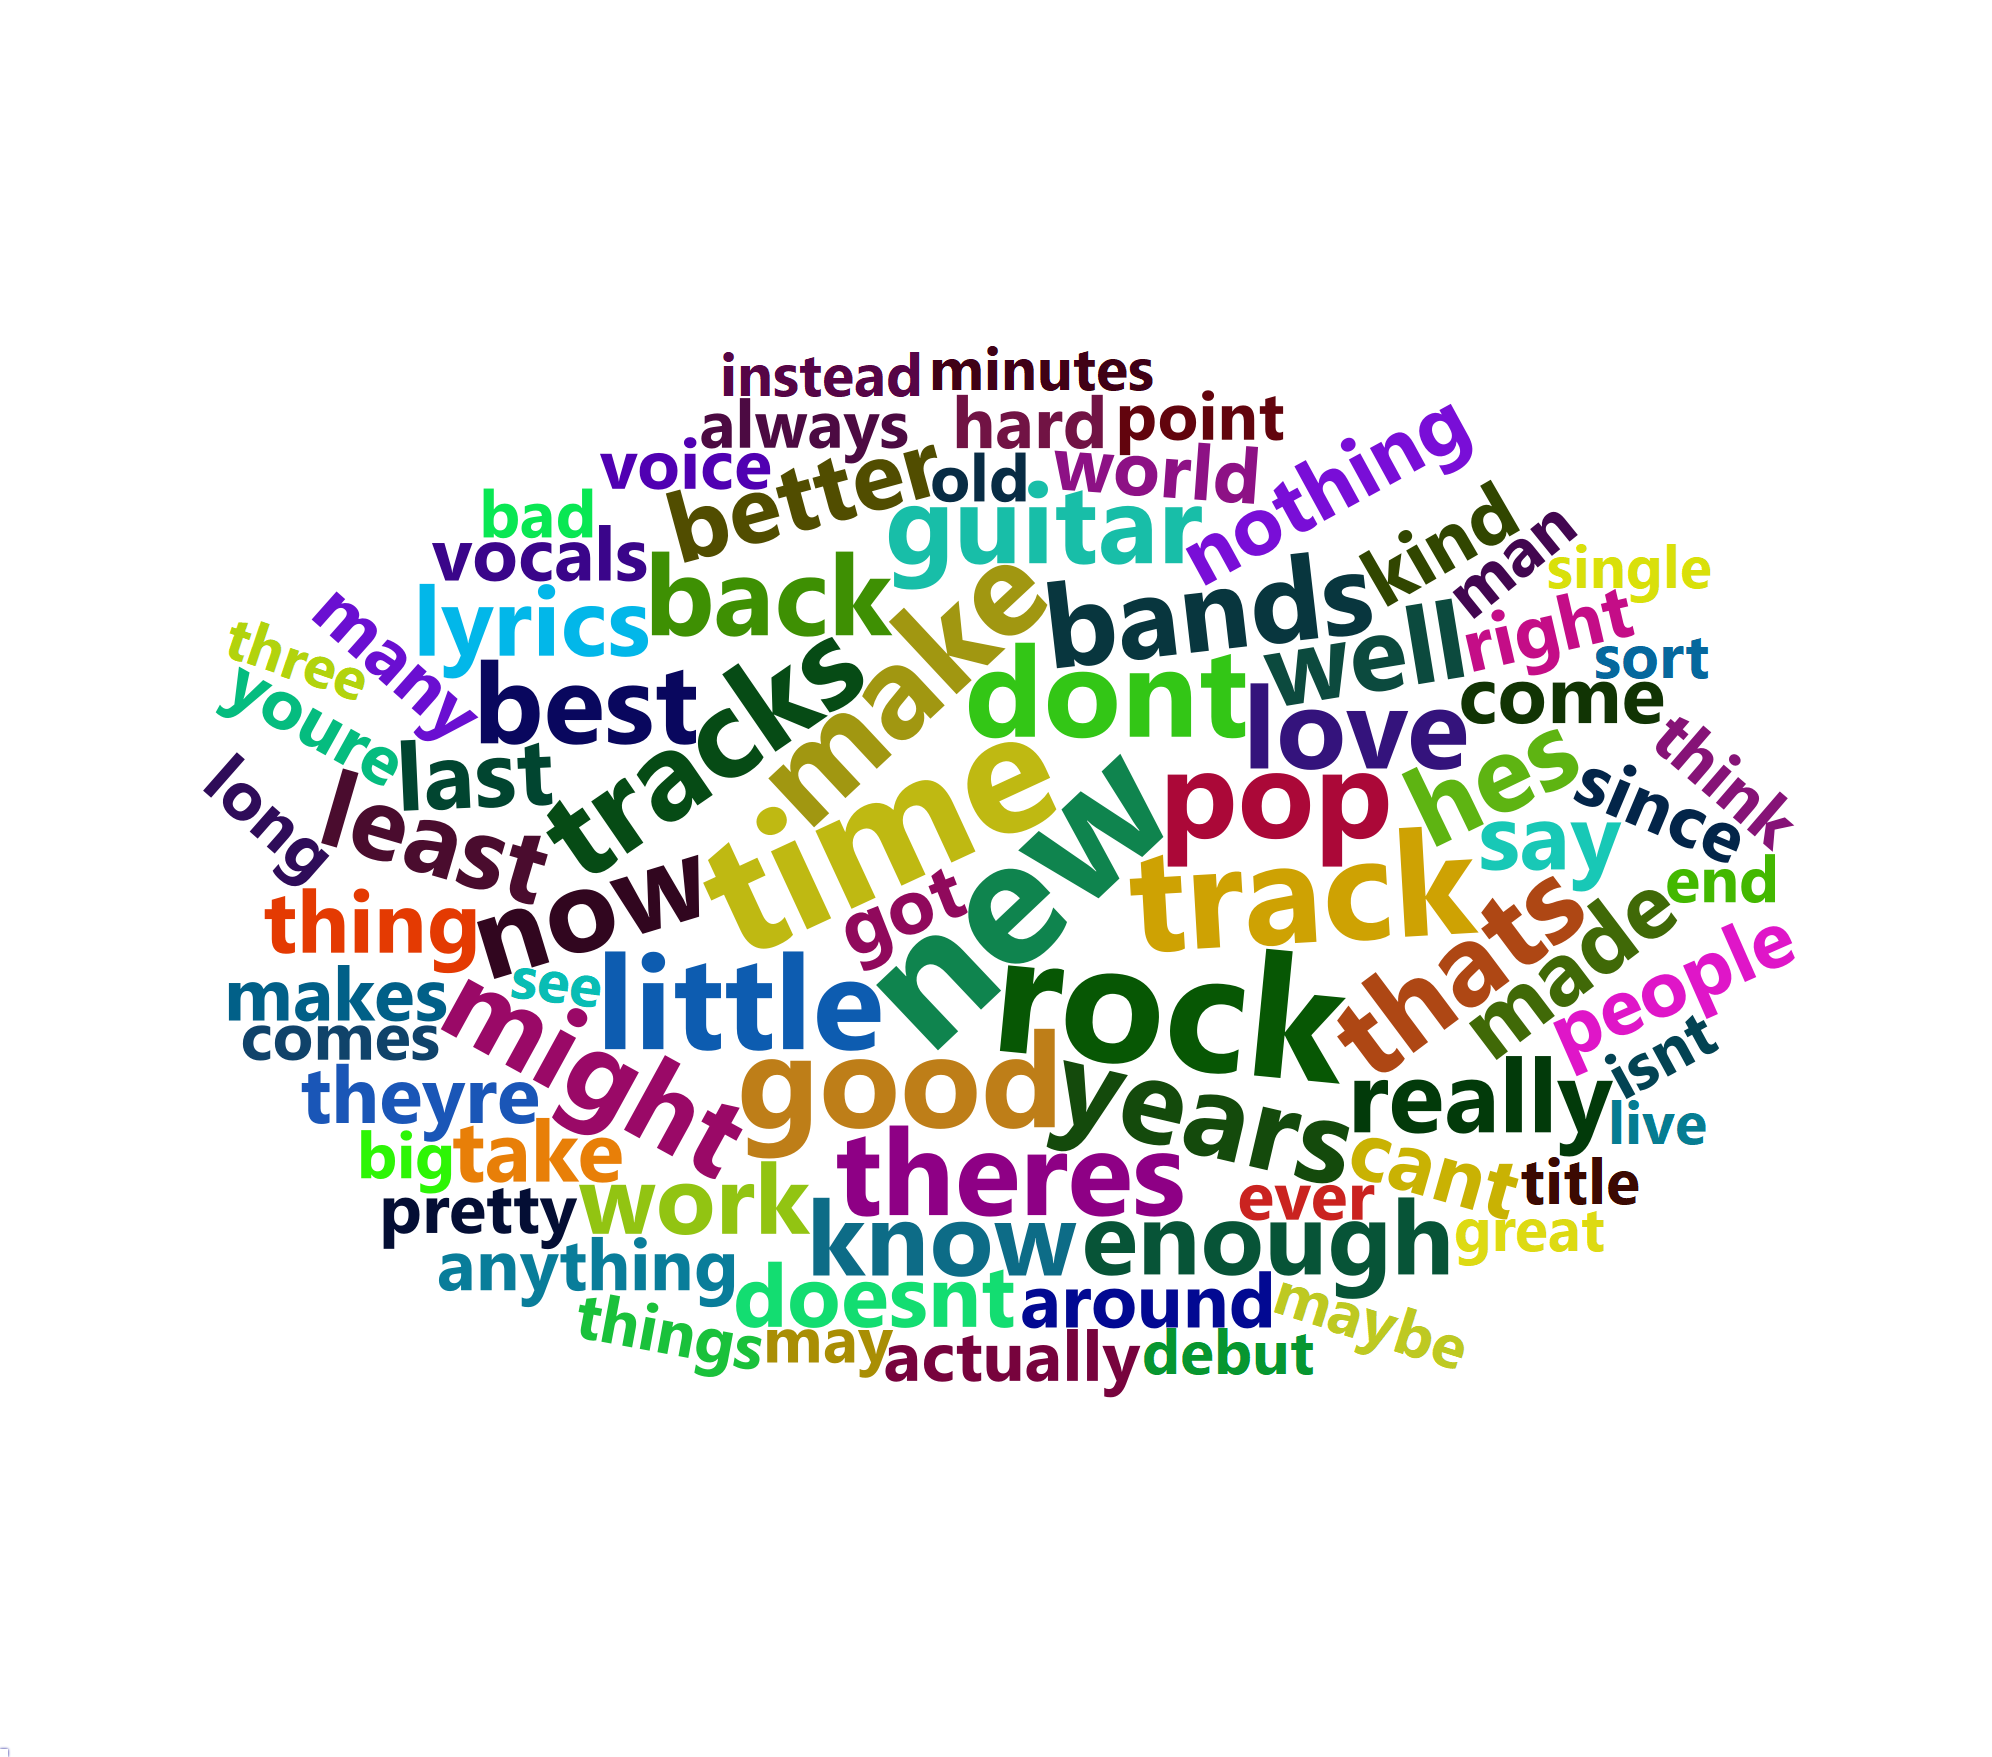
\includegraphics[width = \linewidth]{"figures/wordcloud_bad.png"}
\end{center}











	
\end{document}
